\chapter{Evaluation and benchmarks}
The success of this thesis should be measured on three accounts.
\begin{enumerate}
\item Does the Futhark \csharp{} code generator generate Futhark \csharp{}
  programs that has a performance comparable to the programs that are
  generated by the existing C and Python code generators?

\item Does the \fshark{} language succeed in letting us write GPU kernels in
  declarative \fsharp{} code?
  
\item Does GPU kernels generated from \fshark{} code perform similarly to
  versions implemented in Futhark, and does
\end{enumerate}


\section{The performance of Futhark \csharp{} programs}




\section{The usability and design of the \fshark{} language}

\subsubsection*{Testing arithmetic operators}
For all arithmetic operators available in \fshark{}, I have written an
accompanying test, suitably located in the directory
\texttt{FSharkTests/UnitTests/Operators} in the \fshark{} project.

The test suite for the operators are quite rudimentary, and are primarily
designed to confirm that the types of the operands are preserved when passed to
Futhark \csharp{} and back again.

The test suite does not test edges (such as integer overflows or dividing
decimals by zero) behaves equally in natively executed \fshark{} code and
translated Futhark \csharp{} code.
These edge cases has been left out for SOME reasons.

(THESE ARE NOT ACTUALLY DONE YET)
(Are unit tests enough?)

all convertion functions pass through i64. this might be a mistake, as real
supports f32 to f64

thoughts on correctness of translations
testing correctness of these translations

\subsubsection*{Testing \fsharp{} standard library functions}

\subsubsection*{On comparing floating point values}


\clearpage
\subsection*{The correctness of the \fshark{} subset.}
When transpiling code from one language to another, it is absolutely vital that
the programmer can trust that the target language result
is semantically equivalent to the source language code.

In \fshark{}s case, it means that any program written using the \fshark{}
subset must have the same result no matter whether it is run natively as
\fsharp{} code, or run as \fshark{} compiled Futhark code.

Take for example the logarithm function \texttt{log}. In both \fsharp{} and
Futhark, this function denotes the natural logarithm. If we were translating
from a careless language $l$, where \texttt{log} instead denoted the binary
logarithm, the translation would still be succesfull and not trigger any type
errors.
However, the native result and the Futhark result would be wildly different.

To ensure that every operator and function in the \fshark{} subset has
equivalent results, no matter whether the \fshark{} code is run as native
\fsharp{} code, or compiled into Futhark, I have written a test suite with unit
tests for each element in the \fsharp{} subset. 

An \fshark{} test is an \fshark{} module, but with two extra values added,
namely an input and an output value for the test. For example, the test written for the
division operator is shown in figure \ref{fig:fsharkdivtest}.

\begin{figure}[h]
  \centering
\begin{minted}[breaklines=true, fontsize=\footnotesize]{fsharp}
module Div
open FSharkPrelude.FSharkPrelude
open FShark.TestTypes.TestTypes
open System

[<FSharkEntry>]
let div (fiveByte : int8) (fiveShort : int16) (five : int) 
        (fiveLong : int64) (fiveSingle : single) (fiveDouble : double) 
        : (int8 * int16 * int * int64 * single * double) =

    (fiveByte / 2y, fiveShort / 2s, five / 2, 
     fiveLong / 2L, fiveSingle / 2.0f, fiveDouble / 2.0)

[<FSharkInput>]
let value = [|5y; 5s; 5; 5L; 5.0f; 5.0|] : obj array

[<FSharkOutput>]
let sameValue = 
  (2y, 2s, 2, 2L, 2.5f, 2.5) : (int8 * int16 * int * int64 * single * double)
\end{minted}
  \caption{The unit test for the \fshark{} division operator}
  \label{fig:fsharkdivtest}
\end{figure}


\section{The performance of \fshark{} generated GPU kernels}

Appendices show 
\section*{The \texttt{LocVolCalib} benchmark}
small.in:
FShark (openCL) took 211882 microseconds.
Average invokation (fshark non openCL) time was 81194767 microseconds.
Native took 438 929 311 microseconds.

\begin{figure}
    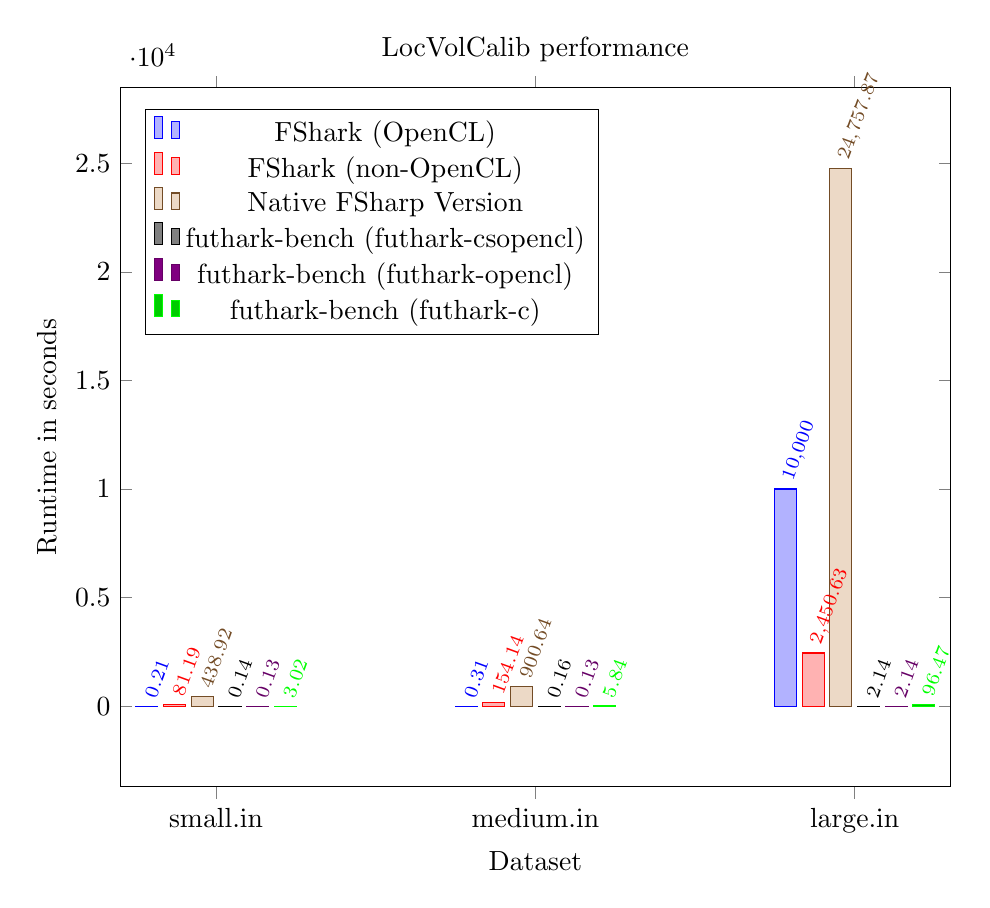
\begin{tikzpicture}
      \begin{axis}[
        title={LocVolCalib performance},
        xlabel={Dataset},
        ylabel={Runtime in seconds},
        width=1\textwidth,
        %height=0.5,
        symbolic x coords={small.in,medium.in,large.in},
        xtick=data,
        enlargelimits=0.15,
        ybar=2pt,% configures ‘bar shift’
        bar width=8pt,
        nodes near coords,
        every node near coord/.append style={rotate=70, anchor=west,font=\scriptsize},
        legend style={legend pos=north west}
      ]
      \addplot plot coordinates {(small.in, 0.21 ) (medium.in, 0.31 ) (large.in, 9999.9999 )};
      \addplot plot coordinates {(small.in, 81.19 ) (medium.in, 154.14 ) (large.in, 2450.63 )};
      \addplot plot coordinates {(small.in, 438.92 ) (medium.in, 900.64 ) (large.in, 24757.87 )};
      \addplot plot coordinates {(small.in, 0.14 ) (medium.in, 0.16 ) (large.in, 2.14 )};
      \addplot plot coordinates {(small.in, 0.13 ) (medium.in, 0.13 ) (large.in, 2.14 )};
      \addplot plot coordinates {(small.in, 3.02 ) (medium.in, 5.84 ) (large.in, 96.47 )};

      \legend{FShark (OpenCL), FShark (non-OpenCL), Native FSharp Version, futhark-bench (futhark-csopencl), futhark-bench (futhark-opencl), futhark-bench (futhark-c)}
      \end{axis}
    \end{tikzpicture}
    \caption{Comparison between Python and Futhark performance for simple model}
    \label{fig:line-graph}
\end{figure}

medium.in:
(Fshark opencl)invokation time was 310833 microseconds
Fshark nonopencl Average invokation time was 154 141 321 ms
Native took 900 643005 microseconds.

large.in:

fshark with opencl Memory Allocation Error
fshark sans opencl 2450 637 053 microseconds
Native took 24757 874 577 microseconds.


for all three datasets
%% master ●  futhark-bench --compiler=futhark-csopencl LocVolCalib.fut 
%%Compiling LocVolCalib.fut...
%%Results for LocVolCalib.fut:
%%dataset LocVolCalib-data/small.in:   143141.00us (avg. of 10 runs; RSD: 0.02)
%%dataset LocVolCalib-data/medium.in:  163246.30us (avg. of 10 runs; RSD: 0.00)
%%dataset LocVolCalib-data/large.in:  2143760.90us (avg. of 10 runs; RSD: 0.00)
%%
%% master ●  futhark-bench --compiler=futhark-opencl LocVolCalib.fut 
%%Compiling LocVolCalib.fut...
%%Results for LocVolCalib.fut:
%%dataset LocVolCalib-data/small.in:   134473.30us (avg. of 10 runs; RSD: 0.02)
%%dataset LocVolCalib-data/medium.in:  134796.20us (avg. of 10 runs; RSD: 0.01)
%%dataset LocVolCalib-data/large.in:  1924412.20us (avg. of 10 runs; RSD: 0.01)

%% master ●  futhark-bench --compiler=futhark-c LocVolCalib.fut     
%%Compiling LocVolCalib.fut...
%%Results for LocVolCalib.fut:
%%dataset LocVolCalib-data/small.in:  3 020588.60us (avg. of 10 runs; RSD: 0.01)
%%dataset LocVolCalib-data/medium.in: 5 842482.00us (avg. of 10 runs; RSD: 0.01)
%%dataset LocVolCalib-data/large.in:  96 476520.00us (avg. of 10 runs; RSD: 0.00)
%%


\section*{The \texttt{nbody} benchmark}

for all three datasets


\subsection*{Specifications for benchmark}
We have run the benchmarks on a system with these attributes:
\begin{itemize}
\item CPU: 4 cores of Intel Core i5-6500 at 3.20GHz
  \begin{itemize}
  \item L1 cache: 128 KiB 
  \item L2 cache: 1024 KiB 
  \item L3 cache: 6144 KiB 
  \end{itemize}
\item GPU: GeForce GTX 970
\end{itemize}


Introduction for the two benchmarks LocVolCalib and nbody



why are they faster in general




%%% Local Variables:
%%% mode: latex
%%% TeX-master: "../thesis"
%%% End: